\documentclass[letterpaper]{article}

\usepackage{aaai}
\usepackage{times}
\usepackage{helvet}
\usepackage{courier}

\frenchspacing
\setlength{\pdfpagewidth}{8.5in}
\setlength{\pdfpageheight}{11in}

%% SZ; for submission only
\setlength{\titlebox}{1.75in}
\nocopyright   

% \usepackage[numbers]{natbib}            % Bibliography
\usepackage{amsmath}                    % For Math Proofs
\usepackage{amsthm}                     % For Math Proofs
\usepackage{amssymb}                    % For Math Proofs
\usepackage{amsfonts}                   % For Math Proofs
\usepackage{algorithm}                  % For Algorithms
\usepackage{algorithmic}                % For Algorithms
\usepackage{graphicx}                   % For Graphics/Figures
\usepackage{float}                      % For Graphics/Figures
\usepackage{epstopdf}                   % Convert eps images to pdf
\usepackage{mathabx}                    % For \bigtimes -- Cartesian product

% Create some formatting and definitions.
\theoremstyle{definition}
\newtheorem{problem}{Problem}
\newtheorem{assumption}{Assumption}
\newtheorem{example}{Example}
\newtheorem{definition}{Definition}
\newtheorem{notation}{Notation}
\newtheorem{theorem}{Theorem}
\newtheorem{corollary}{Corollary}
\newtheorem{remark}{Remark}
\newtheorem{proposition}{Proposition}
\newtheorem{lemma}{Lemma}
\DeclareMathOperator*{\argmin}{argmin}
\DeclareMathOperator*{\argmax}{argmax}
\DeclareMathOperator*{\lvmax}{lvmax}
\DeclareMathOperator*{\leximax}{leximax}
\DeclareMathOperator*{\leximin}{leximin}


\pdfinfo{
/Title (Multi-Objective MDPs with Lexicographic Reward Preferences)
/Author (Kyle Hollins Wray, Shlomo Zilberstein, Abdel-Illah Mouaddib)}

\setcounter{secnumdepth}{1}

\title{Multi-Objective MDPs with Lexicographic Reward Preferences}

\author{AAAI Submission \#}

%\author{Kyle Hollins Wray \and Shlomo Zilberstein \\
%  University of Massachusetts \\
%  Amherst, MA 01003, USA \\
%  {\tt \{wray, shlomo\}@cs.umass.edu} \And
%  Abdel-Illah Mouaddib \\
%  GREYC - Univeaite de Caen \\
%  Bd Marechal Juin, BP 5186 \\
%  F14032 Caen Cedex, France \\
%  {\tt mouaddib@info.unicaen.fr}}


\begin{document}

\maketitle

\begin{abstract}
%\begin{quote}
Sequential decision problems that involve multiple objectives are prevalent.  Consider for example a driver of a semi-autonomous car who may want to minimize both travel time and the effort associated with manual driving.  We introduce a rich model called lexicographic MDP (LMDP) and a corresponding planning algorithm called LVI that generalize previous work by allowing for conditional lexicographic preferences with slack.  We analyze the convergence characteristics of LVI and establish its game theoretic properties. The performance of LVI in practice is tested within a realistic benchmark problem in the domain of semi-autonomous driving. Finally, we demonstrate how GPU-based optimization can improve the scalability of LVI and other value iteration algorithms for MDPs.
%\end{quote}
\end{abstract}



\section{Introduction}
\label{sec:introduction}

% Introduce the premise:
% 1. Interesting / prevalent research area.
% 2. Example problem domains.
% 3. Some of the challenges, hinting that our algorithm addresses these.
% 4. Conclude with a one or two sentence description of our algorithm.
Stochastic planning problems designed to optimize multiple objectives are widespread within numerous domains such as smart homes and commercial buildings~\cite{Kwak12-SAVES}, reservoir water control~\cite{Castelletti08-WaterReservoirControl}, and autonomous robotics~\cite{Mouaddib04-MultiObjectivePathPlanning,Calisi07-MultiObjectiveExplorationAndSearchRobots}. 
Current approaches often use a scalarization function and a weight vector to project the multi-objective problem to a single-objective problem~\cite{Roijers13-SurveyMultiObjective,Natarajan05-DynamicPreferencesMCRL,Perny10-FindingCompromiseSolutionsMOMDPs,Perny13-LorenzOptimalSolutionsMOMDPs}. While these approaches leverage effectively the vast existing work on single-objective optimization, they have several drawbacks.  First, choosing a projection is often too onerous to use in practice since there are many viable Pareto optimal solutions to the original multi-objective problem, making it hard to visualize and analyze alternative solutions. Often there is no clear way to prefer one over another. In some cases, a simple lexicographic order exists among the objectives, for example using plan safety as primary criterion and cost as secondary. But lexicographic order of objectives can be too rigid, not allowing any tradeoffs between objectives (e.g., a large reduction in costs for a minimal reduction in safety).

Recent work by~\citeauthor{Mouaddib04-MultiObjectivePathPlanning} used a strict lexicographic preference ordering for multi-objective MDPs~\cite{Mouaddib04-MultiObjectivePathPlanning}. Others have also developed lexicographic orderings over value functions, calling this technique \emph{ordinal dynamic programming} \cite{Mitten74-PreferenceOrderDynamicProgramming,Sobel75-OrdinalDynamicProgramming}. \citeauthor{Mitten74-PreferenceOrderDynamicProgramming} assumed a specific preference ordering over outcomes for a finite horizon MDP; \citeauthor{Sobel75-OrdinalDynamicProgramming} extended this model to infinite horizon MDPs. Ordinal dynamic programming has been explored under reinforcement learning~\cite{Gabor98-MultiObjectiveReinforcementLearning,Natarajan05-DynamicPreferencesMCRL}, with the notion of a minimum criterion value, distinct from slack. 

We propose a natural extension of sequential decision making with lexicographic order by introducing two added model components: conditioning and slack.  Conditioning allows the lexicographic order to depend on certain state variables.  Slack allows a small deviation from the optimal value of a primary variable so as to improve secondary value functions.  The added flexibility is essential to cature practical preferences in many domains.  For example, in manufacturing, there is always a tradeoff among cost, quality, and time. In critical states of the manufacturing process, one may prefer to optimize quality with no slack, whereas in less important states one may optimize cost, but allow for some slack in order to improve time and quality. 

Our interest in developing this model stems from work on planning for semi-autonomous driving.  Consider a car that can operate autonomously under certain conditions, for example maintaining safe speed and distance from other vehicles on a highway.  All other roiad conditions require manual driving. A driver may want to minimize both the time needed to reach the destination and the effort associated with manual driving. The concepts of conditional preference and slack are quite valuable in defining the overall objective. To ensure safety, if the driver is tired, then selecting roads which are autonomous-capable are preferred without any margin of slack; however, if the driver is not tired, then roads which optimize travel time are preferred, perhaps with some slack to allow for long-distance, autonomous-capable highways. We focus on this domain for the remainder of the paper.


%% [[ a bit misplaced?]]
%Within the context of scalarization methods, Lorenz dominance has been used with weighted value functions to favor more ``fair'' values~\cite{Perny13-LorenzOptimalSolutionsMOMDPs}.

The general use of preference decomposition is popular within the field, as found in Generalized Additive Decomposable (GAI) networks~\cite{Gonzales11-DecisionMakingMultipleObjectivesGAINetworks} or Conditional Preference Networks (CP-Nets)~\cite{Boutilier04-CPNets}. Constrained MDPs (CMDPs) can also capture this preference structure, as well as slack, and are potentially a more general representation than LMDPs~\cite{Altman99-CMDPs}; however, to our knowledge lexicographic preferences have not been explored within the model. Various other forms of slack are also commonly found in the literature~\cite{Gabor98-MultiObjectiveReinforcementLearning}. Combining these ideas, LMDP and LVI naturally encapsulates many problem domains.


%%% [[not needed?]] We introduce the LMDP model and LVI algorithm that generalize these previous methods with our formulation of slack variables and conditional state-based preferences. Additionally, we present experimental evidence, which demonstrates its efficacy in an applied setting. To the best of our knowledge, no other model or algorithm allows for lexicographic state-based conditional preferences or our formulation of slack.

Our primary contributions include formulating the Lexicographic MDP (LMDP) model and the corresponding Lexicographic Value Iteration (LVI) algorithm. They generalize the previous methods mentioned above with our formulation of slack variables and conditional state-based preferences. We also provide an interesting connection between decision theory and game theory, in addition to a statement for the uniqueness of LMDP policies with respect to linearly weighted scalarization function policies. Furthermore, we introduce a new benchmark problem for multi-objective research: semi-autonomous driving. We implement general tools to experiment in this domain, leveraging the OpenStreetMap (OSM) package--a collaborative project to create a free editable map of the world.  Finally, we employ GPU-based optimization to implement our algorithm and show its general benefits for Value Iteration (VI) in MDPs.

Section~\ref{sec:problem_definition} states the LMDP problem definition. Section~\ref{sec:theoretical_analysis} presents our main convergence results, bound on slack, and an interesting relation to game theory. Section~\ref{sec:experimentation} discusses our experimentats within the context of semi-autonomous driving. Finally, Section~\ref{sec:conclusion} concludes with a final discussion of LMDPs and LVI.

% Discuss previous work on multi-objective optimization. Each time, state in 1 sentence what the algorithm does, then "but" with how our algorithm differs.
%Scalarization either assumes the weights are known, which produces a single policy, or allows for the selection of weights, which produces a set of possible Pareto optimal policies~\cite{Roijers13-SurveyMultiObjective}. In both cases, the designer must also select a linear or monotonically increasing scalarization function. We instead explore a lexicographic approach that allows for flexibility with slack. Since the problem domain is assumed to be known, it is natural to prescribe a state-dependent ordering over the rewards. Each action taken optimizes the value functions in order, only referring to the subsequent one if multiple actions exist which yield the optimal value, while allowing for some slack.

% Discuss previous work on the use of lexicographic orderings in MDPs, each time stating in 1 sentence what the approach was and how ours differs.


%\citeauthor{Barbara88-MaxminLeximax} characterized an operator called $\leximin$ within an economics context, which is closely related to $\lvmax$, except that the ordering is slightly different and does not include slack variables~\cite{Barbara88-MaxminLeximax}. Since its inception, it has enjoyed use outside the domain of MDPs by other economics researchers~\cite{Bossert94-RankingOpportunitySets,Fargier05-QuantitativeDecisionMaking,Arlegi05-FreedomOfChoice}.

%Our algorithm can capture the strict avoidance of dead ends as well as loops. Interestingly,~\citeauthor{Kolobov12-TheoryGoalOrientedMDPsDeadEnds} showed that unavoidable dead ends can be represented by a ``price''~\cite{Kolobov12-TheoryGoalOrientedMDPsDeadEnds}. The resulting formulation resembles a specific, non-slack variable version of $\lvmax$ value iteration.

%A solid survey of the approaches used to solve MOMDPs is provided by~\citeauthor{Roijers13-SurveyMultiObjective}~\shortcite{Roijers13-SurveyMultiObjective}, but other models exist. Constrained MDPs (CMDPs) are another formulation of MOMDPs, but to our knowledge no one has explored lexicographic preferences over rewards in this domain~\cite{Altman99-CMDPs}. Additionally,~\citeauthor{Gonzales11-DecisionMakingMultipleObjectivesGAINetworks} used Generalized Additive Decomposable (GAI) networks to capture the decomposability of the utility functions to model preferences~\cite{Gonzales11-DecisionMakingMultipleObjectivesGAINetworks}.



\section{Problem Definition}
\label{sec:problem_definition}

We present a formal model for multi-objective MDPs (MOMDPs) with a lexicographic ordering over the rewards' value functions. An MDP is a stochastic control process in which an agent exists in a set of states. The actions the agent performs in particular state each have a distribution over potential successor states. This transition results in a reward. The process operates over the state space for a finite or (virtually) infinite number of discrete time steps. The goal is to maximize an expected reward over the collection stages. Definition~\ref{def:mdp} formally states this process.
\begin{definition}
    \label{def:mdp}
    A \textbf{Multi-Objective Markov Decision Process (MOMDP) with lexicographic reward preferences} is a represented by a 4-tuple $\langle S, A, T, \mathbf{R} \rangle$ with:
    \begin{itemize}
        \item $S$ is a finite set of $n$ states, with initial state $s_0 \in S$
        \item $A$ is a finite set of $m$ actions
        \item $T : S \times A \times S \rightarrow [0, 1]$ is a state transition function which specifies the probability of transitioning from a state $s \in S$ to state $s' \in S$, given action $a \in A$ was performed; equivalently, we may write $T(s, a, s') = Pr(s' | s, a)$
        \item $\mathbf{R} = [R_1, \ldots, R_k ]^T$ is a vector of reward functions $R_i : S \times A \times S \rightarrow \mathbb{R}$, $\forall i \in K$, with $K = \{1, \ldots, k\}$; each specifies the reward for being in a state $s \in S$, performing action $a \in A$, and transitioning to a state $s' \in S$, often written as $\mathbf{R}(s, a, s') = [R_1(s, a, s'), \ldots, R_k(s, a, s')]^T$
    \end{itemize}
\end{definition}

We call $h \in \mathbb{N} \cup \{ \infty \}$ the \emph{horizon}, i.e., number of steps until the process terminates. The process may be defined as finite ($h < \infty$) or infinite ($h = \infty$). Over the iterations, rewards are discounted by \emph{discount factor} $\gamma$. For finite horizon problems, typically $\gamma = 1$; for infinite horizon problems, $\gamma \in [0, 1)$.

A \emph{policy} $\pi : S \rightarrow A$ is a mapping from each state $s \in S$ to an action $a \in A$. In finite horizon problems, we have a sequence of policies $\langle \pi_1, \ldots, \pi_h \rangle$ representing a policy for each stage.

Let $\mathbf{V} = [V_1, \ldots, V_k]^T$ be a set of \emph{value functions}. Let each function $V_i^\pi : S \rightarrow \mathbb{R}$, $\forall i \in K$, represent the value of states $S$ following policy $\pi$. The stochastic process of MDPs enable us to represent this using the expected value over the reward for following the policy at each stage.
\begin{equation*}
    \mathbf{V}^\pi(s) = \mathbb{E} \Big[ \sum_{t=0}^{h-1} \gamma^t \mathbf{R}(s^t, \pi(s^t), s^{t+1}) \Big| s^0 = s, \pi \Big]
\end{equation*}

This allows us to recursively write the value of the state $s \in S$, given a particular policy $\pi$, in the following manner.
\begin{equation*}
    \mathbf{V}^\pi(s) = \sum_{s' \in S} T(s, \pi(s), s') (\mathbf{R}(s, \pi(s), s') + \gamma \mathbf{V}^\pi(s'))
\end{equation*}
% The final policy $\pi$ is computed using the value function.
% \begin{equation}
%     \pi(s) = \argmax_{a \in A} \mathbf{V}...
% \end{equation}


\subsection{Lexicographic Value Iteration}

We lexicographically prefer $V_i^\pi$ to $V_{i+1}^\pi$ for each $i \in K$. We are able to rewrite value iteration to solve multi-objective MDPs in this manner. In particular, the $\max$ operator needs to be replaced with a \emph{lexicographic vector maximization} operator, denoted $\lvmax$, which is defined in its general form in Definition~\ref{def:lvmax} below.

\begin{definition}
\label{def:lvmax}
The \textbf{lexicographic vector maximization} operator $\lvmax$ is defined in Equation~\ref{eq:lvmax} below. Let $X$ be a set and $f : X \rightarrow \mathbb{R}^k$ be a vector function. Let $\delta \in \mathbb{R}_+^k$ be a tuple of non-negative slack variables. Let $X_1 = X$ and increasingly smaller subsets of $X$ as
\begin{equation}
    \label{eq:lvmax_X}
    X_{i+1} = \{x \in X_i | \max_{x' \in X_i} f_i(x') - f_i(x) \leq \delta_i \}
\end{equation}
for all $i \in \{1, \ldots, k-1\}$. To break ties, we define the final subsets as $X_1^* = X_k$ and $X_{i+1}^* = \argmax_{x \in X_i^*} f_i(x)$.

\begin{equation}
    \label{eq:lvmax}
    \lvmax_{x \in X} \mathbf{f}(x) = \begin{bmatrix}
            \max_{x \in X_1^*} f_1(x) \\
            \vdots \\
            \max_{x \in X_k^*} f_k(x)
        \end{bmatrix}
\end{equation} 
\end{definition}

With this definition, the \emph{Bellman update equation} for MOMDPs with lexicographic reward preferences may be written as Equation~\ref{eq:lvmax_value_iteration} below for all states $s \in S$.
\begin{align}
    \mathbf{V}(s) &= \lvmax_{a \in A} \mathbf{Q}(s, a) \label{eq:lvmax_value_iteration} \\
    \mathbf{Q}(s, a) &= \sum_{s' \in S} T(s, a, s') (\mathbf{R}(s, a, s') + \gamma \mathbf{V}(s')) \label{eq:lvmax_Q}
\end{align}
This operator will only converge to within $\mathbf{\delta}$ of the actual value of the states.


\section{Theoretical Analysis}
\label{sec:theoretical_analysis}

We provide a proof of convergence for $\lvmax$ value iteration in Proposition~\ref{prop:lvmax_convergence}.

\begin{proposition}
    \label{prop:lvmax_convergence}
    Lexicographic vector max ($\lvmax$) value iteration converges to a unique fixed point of value functions, given discount factors $\gamma_i \in [0, 1)$ for all $i \in K$ and \emph{Lipschitz constant} $\nu \in [0, 1)$ defined as
    \begin{equation}
        \label{eq:lvmax_convergece_nu}
        \nu = \max_{i \in K} \Big( \gamma_i + (1 - \gamma_i) \frac{\delta_i}{|R_i^+ - R_i^-|} \Big)
    \end{equation}
    with $R_i^+ = \max_{s \in S} \max_{a \in A} \max_{s' \in S} R_i(s, a, s')$ and $R_i^- = \min_{s \in S} \min_{a \in A} \min_{s' \in S} R_i(s, a, s')$.
\end{proposition}

\begin{proof}
To prove convergence, we must show that the Bellman optimality equation converges to a unique fixed point. We will do this by induction on $i \in K$. First, we must state some definitions.

For a metric space $\langle X, d \rangle$, where $X$ is a set and $d$ is a distance metric, a map $f : X \rightarrow X$ is called a \emph{contraction map} if there exists an $\alpha$ such that $d(f(x), f(y)) = \alpha d(x, y)$, for all $x, y \in X$.

Let the space $X_i$ be the \emph{space of value functions for $i \in K$}, i.e., we have $V_i = [V_i(s_1), \ldots, V_i(s_n)]^T \in X_i$. Let the distance metric $d_i$ be the \emph{max norm}, i.e., $\|V_i\|_\infty = \max_{s \in S} |V_i(s)|$. Since $\gamma_i \in [0, 1)$, the metric space $M_i = \langle X_i, d_i \rangle$ is a \emph{complete metric space}; every Cauchy sequence of $M_i$ converges to a point in $M_i$.

Let the $\lvmax$ Bellman optimality equation's (Equation~\ref{eq:lvmax_value_iteration}) be defined as an operator $B$, i.e., $V^{t+1} = B V^t$, for $V^t, V^{t+1} \in X$ with $t \geq 0$. Let element $i \in K$ of the operator be $B_i$, such that $V_i^{t+1} = (B V^t)_i = B_i V_i^t$. We prove the operator $B_i$ is a contraction map in $M_i$ for all $i \in K$, given either that $i=1$ or that the previous $i-1$ has converged to within $\epsilon$ of its fixed point.

Let $V_{1i}, V_{2i} \in X_i$ be any two value function vectors, and $\gamma_i \in [0, 1)$. We first apply the definition of $\lvmax$ from Equation~\ref{eq:lvmax}.
\begin{equation*}
    \| B_i V_{1i} - B_i V_{2i} \|_\infty = \max_{s \in S} | \max_{a \in A_{1i}^*} Q_{1i}(s, a) - \max_{a \in A_{2i}^*} Q_{2i}(s, a) |
\end{equation*}

By Definition~\ref{def:lvmax}, $A_{1i}^* \subseteq A_{1i}$. Therefore, for all $s \in S$, $\max_{a \in A_{1i}^*} Q_{1i}(s, a) \leq \max_{a' \in A_{1i}} Q_{1i}(s, a)$. Also by Definition~\ref{def:lvmax}, for all $a^* \in A_{2i}^* \subseteq A_{2,i+1} = \{a \in A_{2i} | \max_{a' \in A_{2i}} Q_{2i}(s, a') - Q_{2i}(s, a) \leq \delta_i \}$. Thus,
\begin{align*}
    \max_{a' \in A_{2i}} Q_{2i}(s, a') - \delta_i &\leq Q_{2i}(s, a^*) \leq \max_{a' \in A_{2i}^*} Q_{2i} (s, a') \\
    -\max_{a' \in A_{2i}^*} Q_{2i} (s, a') &\leq \delta_i - \max_{a' \in A_{2i}} Q_{2i}(s, a')
\end{align*}

Without loss of generality, assume that $B_i V_{1i} \geq B_i V_{2i}$, making the absolute value optional in the first equation below. If the opposite is true, then we may simply switch the logic for deriving the two above upper bounds and apply those instead throughout.

Combine these three facts, and we obtain the following.
\begin{align*}
    &\| B_i V_{1i} - B_i V_{2i} \|_\infty \\
    &\leq \max_{s \in S} | \max_{a \in A_{1i}} Q_{1i}(s, a) - \max_{a \in A_{2i}} Q_{2i}(s, a) + \delta_i | \\
    &\leq \max_{s \in S} | \max_{a \in A_{1i}} Q_{1i}(s, a) - \max_{a \in A_{2i}} Q_{2i}(s, a)| + |\delta_i|
\end{align*}

By Definition~\ref{def:lvmax}, when $i=1$ we have $A_{1i} = A_{2i} = A$. Similarly, when $i \in \{2, \ldots, k\}$ given that $i-1$ has converged to within $\epsilon$ of its fixed point, it yields a unique fixed set of actions $A'$, with $A_{1i} = A_{2i} = A' \subseteq A$. Let us denote this fixed actions set as $\bar{A}_i$ for all $i \in K$. Also, as part of the $Q(\cdot)$ values, we distribute $T(\cdot)$ to each $R(\cdot)$ and $V(\cdot)$ in the summations, then apply the property: $\max_x f(x) + g(x) \leq \max_x f(x) + \max_x g(x)$, twice.
\begin{align*}
    &\| B_i V_{1i} - B_i V_{2i} \|_\infty \\
    &\leq \max_{s \in S} \Big| \max_{a \in \bar{A}_i} \Big( \sum_{s' \in S} T(s, a, s') R_i(s, a, s') \\
    &\quad \quad + \gamma_i \sum_{s' \in S} T(s, a, s') V_{1i}(s') \Big) \\
    &\quad \quad - \max_{a \in \bar{A}_i} \Big( \sum_{s' \in S} T(s, a, s') R_i(s, a, s') \\
    &\quad \quad - \gamma_i \sum_{s' \in S} T(s, a, s') V_{2i}(s') \Big) \Big| + \delta_i \\
    &\leq \max_{s \in S} \Big| \max_{a \in \bar{A}_i} \sum_{s' \in S} T(s, a, s') R_i(s, a, s') \\
    &\quad \quad + \gamma_i \max_{a \in \bar{A}_i} \sum_{s' \in S} T(s, a, s') V_{1i}(s') \\
    &\quad \quad - \max_{a \in \bar{A}_i} \sum_{s' \in S} T(s, a, s') R_i(s, a, s') \\
    &\quad \quad - \gamma_i \max_{a \in \bar{A}_i} \sum_{s' \in S} T(s, a, s') V_{2i}(s') \Big| + \delta_i \\
    &\leq \max_{s \in S} \Big| \gamma_i \max_{a \in \bar{A}_i} \sum_{s' \in S} T(s, a, s') V_{1i}(s') \\
    &\quad \quad - \gamma_i \max_{a \in \bar{A}_i} \sum_{s' \in S} T(s, a, s') V_{2i}(s') \Big| + \delta_i
\end{align*}
Note that we can pull out $\gamma_i \in [0, 1)$. Recall, that for any two functions $f$ and $g$, $| \max_x f(x) - \max_x g(x) | \leq \max_x | f(x) - g(x) |$.
\begin{align*}
    &\| B_i V_{1i} - B_i V_{2i} \|_\infty \\
    &\leq \gamma_i \max_{s \in S} \max_{a \in \bar{A}_i} \Big| \sum_{s' \in S} T(s, a, s') (V_{1i}(s') - V_{2i}(s')) \Big| + \delta_i
\end{align*}

Since $\sum_{s' \in S} T(s, a, s') = 1$ and for all $s' \in S$, $T(s, a, s') \in [0, 1]$, it is defined on the $n$-simplex. It then scales the vertices by the values $R(\cdot)$ or $V(\cdot)$. This forms simple convex polytope. Convex polytopes obtain their maximum value at the vertices (or on an entire edge or face, which includes the vertices). Therefore, we may exclusively maximize over these vertices ($R(\cdot)$ and $V(\cdot)$), and may simply drop both maximizations which select the weights (i.e., maximization over $s \in S$ and $a \in A$).
\begin{align*}
    &\| B_i V_{1i} - B_i V_{2i} \|_\infty \leq \gamma_i \max_{s' \in S} \Big| V_{1i}(s') - V_{2i}(s') \Big| + \delta_i \\
    &\leq \gamma_i \| V_{1i} - V_{2i} \|_\infty + \delta_i \frac{\| V_{1i} - V_{2i} \|_\infty}{\| V_{1i} - V_{2i} \|_\infty} \\
    &\leq \Big( \gamma_i + \frac{\delta_i}{\| V_{1i} - V_{2i} \|_\infty} \Big) \| V_{1i} - V_{2i} \|_\infty
\end{align*}

We can place a constant upper bound on this value to remove the denominator $\| V_{1i} - V_{2i} \|_\infty$. Consider any finite or finite sequence of states and actions performed by the agent: $z = \langle s^0, a^0, s^1, a^1, \ldots \rangle$. The utility $u_i^h(z)$ at horizon $h \in \mathbb{N} \cup \{ \infty \}$ is bounded:
\begin{align*}
    u_i^h(\langle s^0, a^0, s^1, a^1, \ldots \rangle) &= \sum_{t=0}^h \gamma_i^t R_i(s^t, a^t, s^{t+1}) \\
        &\leq \sum_{t=0}^\infty \gamma_i^t R_i^+ \leq \frac{R_i^+}{1 - \gamma_i}
\end{align*}
Similarly,
\begin{equation*}
    -u_i^h(\langle s^0, a^0, s^1, a^1, \ldots \rangle) \geq \frac{R_i^-}{1 - \gamma_i}
\end{equation*}
The value function is therefore bounded by these values, because including state transitions would only decrease the values.
\begin{align*}
    \| V_{1i} - V_{2i} \|_\infty &\leq \Big| \frac{R_i^+}{1 - \gamma_i} - \frac{R_i^-}{1 - \gamma_i} \Big| \leq \frac{|R_i^+ - R_i^-|}{1 - \gamma_i} \\
    \Rightarrow \quad \quad \frac{-1}{\| V_{1i} - V_{2i} \|_\infty} &\leq -\frac{1 - \gamma_i}{|R_i^+ - R_i^-|}
\end{align*}

Now we may obtain final result, proving that the Bellman operator $B_i$ is a contraction map on metric space $M_i$, for all $i \in K$.
\begin{align*}
    &\| B_i V_{1i} - B_i V_{2i} \|_\infty \leq \Big( \gamma_i - \delta_i \frac{-1}{\|V_{1i} - V_{2i}\|_\infty}  \Big) \| V_{1i} - V_{2i} \|_\infty \\
    &\leq \Big( \gamma_i - \delta_i \Big( -\frac{1 - \gamma_i}{|R_i^+ - R_i^-|} \Big) \Big) \| V_{1i} - V_{2i} \|_\infty \\
    &\leq \Big( \gamma_i + (1 - \gamma_i) \frac{\delta_i}{|R_i^+ - R_i^-|} \Big) \| V_{1i} - V_{2i} \|_\infty \\
    &\leq \nu \| V_{1i} - V_{2i} \|_\infty
\end{align*}

Thus, for all $i \in K$, by definition of a contraction map, $B_i$ admits at most one fixed point. Additionally, since $M_i$ is a complete metric space, we can guarantee convergence to a unique fixed point. \emph{Banach's fixed point theorem} states that if $M_i = \langle X_i, d_i \rangle$ is a complete metric space and $B_i: X_i \rightarrow X_i$ is a contraction map, then $B_i$ admits a unique fixed point $V_i^* \in X_i$, i.e., $B_i V_i^* = V_i^*$. Thus, we will have convergence of value iteration to a unique fixed point $V_i^* \in X_i$, for all $i \in K$.
\end{proof}

We may also derive an equation which guarantees convergence to within $\epsilon > 0$ of the fixed point, as shown in Proposition~\ref{prop:lvmax_convergence_check}.

\begin{proposition}
    \label{prop:lvmax_convergence_check}
    Lexicographic vector max ($\lvmax$) value iteration converges to within $\epsilon > 0$ of its unique fixed point once $\| V^{t+1} - V^t \|_\infty < \epsilon \frac{1 - \nu}{\nu}$.
\end{proposition}

\begin{proof}
From Proposition~\ref{prop:lvmax_convergence}, for all $i \in K$, a corollary of Banach's fixed point theorem is that the speed of convergence to within $\epsilon > 0$ of the fixed point $x^*$ is known (using the generic notation from above for a metric space).
\begin{align*}
    d(x^*, x_{t+1}) &\leq \frac{\alpha}{1 - \alpha} d(x_{t+1}, x_t) \\
    \| V_i^* - V_i^{t+1}\|_\infty &\leq \frac{\nu}{1 - \nu} \| V_i^{t+1} - V_i^t \|_\infty
\end{align*}

Since we want the distance from the fixed point $V_i^* \in X_i$ to be $\epsilon$, we may rewrite the equation accordingly.
\begin{align*}
    \epsilon &\leq \frac{\gamma_i}{1 - \gamma_i} \| V_i^{t+1} - V_i^t \|_\infty \\
    \epsilon \frac{1 - \gamma_i}{\gamma_i} &\leq \| V_i^{t+1} - V_i^t \|_\infty
\end{align*}
The above equation states that we are at least $\epsilon$ (or more) away from the fixed point when the maximum difference (over the states) between iterations satisfies the inequality. Therefore, we flip the inequality to create a convergence criterion, which ensures that we are $\epsilon$ or less from the fixed point. Finally, this must be true for all $i \in K$, so we may rewrite it with the infinity norm defined over both $K$ and $S$.
\begin{equation*}
    \quad \| V^{t+1} - V^t \|_\infty < \epsilon \frac{1 - \nu}{\nu}
\end{equation*}
\end{proof}

It is straightforward to show that $\lvmax$ value iteration generalizes value iteration, as shown in Proposition~\ref{prop:lvmax_generalizes_vi}.
\begin{proposition}
    \label{prop:lvmax_generalizes_vi}
    Lexicographic vector max ($\lvmax$) value iteration generalizes value iteration.
\end{proposition}

\begin{proof}
Let $M = \langle S, A, T, \mathbf{R} \rangle$ with $\mathbf{R} = \langle R_1 \rangle$ and $\delta_1 = 0$. By Definition~\ref{def:lvmax}, for all $s \in S$, $\mathbf{V}(s) = \lvmax_{a \in A} \mathbf{Q}(s, a) = \max_{a \in A_1^*} Q_1(s, a)$. Since $A_1^* = A_k = A_1 = A$, we have $V_1(s) = \max_{a \in A} Q_1(s, a)$. This is value iteration on $M' = \langle S, A, T, R_1 \rangle$.
\end{proof}

Typically, a multi-objective optimization problem converts the problem into a objective function by summing the value function and weighting them in a particular manner. Our $\lvmax$ value iteration returns a different solution from the linearly weighted function approaches used to solve MOMDPs. Proposition~\ref{prop:lvmax_different_solution} proves this fact.

% Let the set of all policies returned by value iteration operator $B$ be denoted as $\Pi_B$. Formally, we say that the value iteration operator $B$ is \emph{unique} with respect to value iteration operator $B'$, if and only for some $\epsilon > 0$ and $\gamma_i \in [0, 1)$ in MDP $M = \langle S, A, T, R \rangle$, $\Pi_B \not\subseteq \Pi_{B'}$ and $\Pi_{B'} \not\subseteq \Pi_B$.

% \begin{proposition}
%     \label{prop:lvmax_uniqueness}
%     For $\epsilon > 0$ and $\gamma \in [0, 1)$, let $\Pi_{vi}$ be the set of all policies returned by value iteration operator $B_{vi}$ using a weighted objective function with weights $\mathbf{w} \in \mathbb{R}^k$. Also, let $\Pi_{lv}$ be the set of all policies returned by value iteration operator $B_{lv}$ as defined by Equation~\ref{eq:lvmax_value_iteration} with $\epsilon$ and $\gamma$. $B_{lv}$ is unique with respect to $B_{vi}$.
% \end{proposition}

% \begin{proof}
% By the definition of uniqueness, must show that there exists an MDP $M = \langle S, A, T, R \rangle$ such that $\Pi_{vi} \not\subseteq \Pi_{lv}$ and $\Pi_{lv} \not\subseteq \Pi_{vi}$. Assume by contradiction that $\forall M$, $\Pi_{vi} \subseteq \Pi_{lv}$ or $\Pi_{lv} \subset \Pi_{vi}$.

% \end{proof}


\begin{proposition}
    \label{prop:lvmax_different_solution}
    Let the normal Bellman's equation, with linear weights $\mathbf{w} \in \bigtriangleup^k$, and $\lvmax$'s value iteration's resulting value functions be denoted as the $n$-by-$k$ matrices $V^*$ and $V_{lv}^*$, respectively. There exist a class of MOMDPs $\mathcal{M}$ such that $V^* \neq V_{lv}^*$.
\end{proposition}

\begin{proof}
Assume by contradiction that for all $M \in \mathcal{M}$, $V^* = V_{lv}^*$, i.e., there always exists a set of weights $\mathbf{w} \in \bigtriangleup^k$ which makes this so. We know three things for all $s \in S$: $V_{\mathbf{w}}^*(s) = B V_{\mathbf{w}}^*(s)$, $V_{\mathbf{w}}^*(s) = \mathbf{w} \mathbf{V}^*(s)$, and $\mathbf{V}_{lv}^*(s) = B_{lv} \mathbf{V}_{lv}^*(s)$. Therefore, we have:
\begin{align*}
    f(\mathbf{V}_{lv}^*(s), \mathbf{w}) &= f(\mathbf{V}^*(s), \mathbf{w}) = V_{\mathbf{w}}^*(s) = B V_{\mathbf{w}}^*(s) \\
        &= B( f(\mathbf{V}^*(s), \mathbf{w})) = B (f(B_{lv} \mathbf{V}_{lv}^*(s), \mathbf{w}))
\end{align*}
We now apply the Bellman optimality operator to the right side, as well as the $\lvmax$ operator.
\begin{align*}
    f(\mathbf{V}_{lv}^*(s), \mathbf{w}) &= \max_{a \in A} \Big( \sum_{s' \in S} T(s, a, s') f(\mathbf{R}(s, a, s'), \mathbf{w}) \\
        &+ \gamma \sum_{s' \in S} T(s, a, s') f(\max_{a' \in A_i^*} \mathbf{Q}_{lv}^*(s', a'), \mathbf{w}) \Big)
\end{align*}
Apply the properties the linearity of $f$.
\begin{align*}
    0 &= \max_{a \in A} f\Big( \sum_{s' \in S} T(s, a, s') \mathbf{R}(s, a, s') \\
        &+ \gamma \sum_{s' \in S} T(s, a, s') \max_{a' \in A_i^*} \mathbf{Q}_{lv}^*(s', a') - \mathbf{V}_{lv}^*(s), \mathbf{w} \Big) \\
    0 &= \max_{a \in A} f\Big( \mathbf{x}_a, \mathbf{w} \Big)
\end{align*}
Since $\mathbf{w} \in \bigtriangleup^k$, and $f$ is a linear sum of weights and components, we will show that $\exists M \in \mathcal{M}$ such that $\exists s \in S$ such that $\forall i \in K$, $\mathbf{x}_a > 0$.
\end{proof}


\begin{proposition}
    \label{prop:lvmax_dead_end_avoidance}
    Let $M = \langle S, A, T, \mathbf{R} \rangle$, with $\mathbf{R} = \langle R_1, R_2 \rangle$, be a MOMDP with dead ends for $R_1$ and goal states for $R_2$. Assume there exists a proper policy. With $\gamma = 1$, $\lvmax$ value iteration converges to a policy which strictly avoids dead ends, and otherwise strictly prefers goal states.
\end{proposition}



\section{Experimentation}
\label{sec:experimentation}

This section is just to provide some initial experiments.

\subsection{Grid World with Dead Ends}
First, we implemented a model similar to the classic grid world problem. The agent may move north, south, east, and west in a $w$-by-$h$ grid world. The agent moves successfully with a $0.8$ probability, and fails by moving right or left, each with a $0.1$ probability. At the edges, if the agent cannot move, it remains still.

Throughout the area, dead ends are placed (denoted by ``-'') as well as goal states (denoted by ``+''). In the normal MDP version, dead ends have a reward of $-\infty$, and only have a positive weight of $1.0$ on the transition probability for remaining in the dead end. Goal states have a reward of $1.0$, and all other states have a small penalty of $-0.03$.

In our MOMDP with lexicographic reward function model, we separate the dead ends and goal states into two reward functions. The first reward $R_1$ provides a $0.0$ reward for all states, and a $-1.0$ reward for transitioning to a dead end. The second reward $R_2$ yields a $1.0$ for transitioning to a goal state, and a $-0.03$ for all other states.

We implemented this initial test in Python 2.7. Figures~\ref{fig:seed_1},~\ref{fig:seed_2}, and~\ref{fig:seed_3} show some example output from the model in this domain. Interestingly, it appears to work very well at strictly avoiding dead ends, and then optimizing around the remaining action possibilities.
\begin{figure}[h]
    \centering
    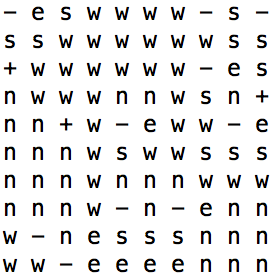
\includegraphics[width=0.4\textwidth,bb=0 0 279 280]{seed_1.png}
    \caption{First example's policy.}
    \label{fig:seed_1}
\end{figure}

\begin{figure}[h]
    \centering
    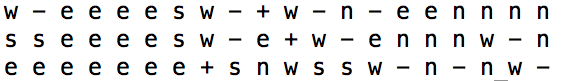
\includegraphics[width=0.4\textwidth,bb=0 0 561 81]{seed_2.png}
    \caption{Second example's policy.}
    \label{fig:seed_2}
\end{figure}

\begin{figure}[h]
    \centering
    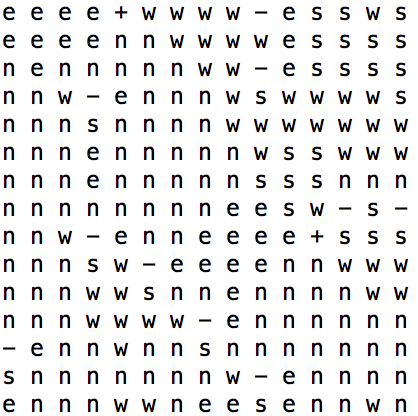
\includegraphics[width=0.4\textwidth,bb=0 0 418 416]{seed_3.png}
    \caption{Third example's policy.}
    \label{fig:seed_3}
\end{figure}

There are additional scenarios for which $\lvmax$ is useful. If there are primary and secondary goals, they can be represented by different rewards, with primary goal states strictly favored over secondary goal states.

\begin{itemize}
    \item If there exists a perfect policy, then it seems to always converge with $\gamma = 1$. The convergent policy always strictly avoids the dead ends, as desired.
    \item Without a perfect policy, it converges but the policy can often be off if a lot of dead ends are close to one another. This is probably one example where the slack variables $\delta_1, \ldots, \delta_k$ could be useful.
    \item These results do not utilize the slack variables: $\delta_1, \ldots, \delta_k$.
\end{itemize}


\subsection{Multi-Objective Autonomous Driving}

To demonstrate the usefulness of both the lexicographic ordering as well as the slack variables, we are considering the autonomous driving domain. We will consider a path planning agent acting over an OpenStreetMap graph, which strictly prefers: shorter time/distance $>$ saving fuel/money $>$ stopping at optional amenities.

Our agent has some slack in optimizing the distance traveled. This allows for it to take an extra 5 minutes to go a bit out of the way in order to save some fuel, or stop at an optional amenity. This same slack holds for the other value functions as well.

We also can model dead ends in this domain. Consider an agent that can choose to drive faster. This might result in a ticket if they drive too fast an get caught, which could be considered a dead end.

This is currently being developed in C++, with supporting scripts to read the OpenStreetMap (OSM) file format written in Python.


%\section{Discussion}
\label{sec:discussion}


\section{Conclusion}
\label{sec:conclusion}


Definitions:
1. Novel model for conditional lexicographic MDPs.
2. Novel algorithm to solve this model based on VI.


Proofs:
1. Formal worst-case bound for slack.
2. Completeness by the convergence for a subset of LMDPs which satisfy an assumption. We also explained exactly why this assumption exists.
3. Correctness of LMDPs and LVI, in terms of its connection to a normal form game.
4. Uniqueness and novelty of the resulting policy as compared to linearly weighted scalarization functions.


Experimentation:
1. Natural use in a novel domain for semi-autonomous systems.
2. Addressed scalability issues via GPU-based optimizations.


Future Work:
1. Convergence of LVI in the general case, for which our simulations suggest must exist. Also, since it is related to a Nash equilibrium, it must be a fixed point.
2. Detailed discussion of GPU-based optimizations for LVI.
3. A complete definition of semi-autonomous systems, and a set of corresponding experiments using LMDPs and LVI.



\section{Acknowledgements}
\label{sec:acknowledgements}



\newpage

\bibliographystyle{aaai}
\bibliography{references}

\newpage

\section*{Supplement to Submission \#}
\label{sec:supplement}

This section includes supplemental material for the paper.

Proof of {\bf Proposition~\ref{prop:lvi_eta_convergence_check}}:
\begin{proof}
Expanding upon Proposition~\ref{prop:lvi_contraction}, for all $i \in K$, by definition of a contraction map, $B_i$ admits at most one fixed point. By \emph{Banach's fixed point theorem}, since $M_i$ is a complete metric space and $B_i$ is a contraction map on $Y_i$, $B_i$ admits a unique fixed point $V_i^* \in Y_i$. Therefore, the final $V^*$ is a unique fixed point in the space over all value functions over $i \in K$ and $s \in S_j$.

Finally, a corollary of Banach's fixed point theorem is that the speed of convergence to within $\epsilon > 0$ of the fixed point $x^*$ is known (using the generic notation from above for a metric space).
\begin{align*}
    d(x^*, x_{t+1}) &\leq \frac{\alpha}{1 - \alpha} d(x_{t+1}, x_t) \\
    \| V_i^* - V_i^{t+1}\|_\infty^{S_j} &\leq \frac{\gamma}{1 - \gamma} \| V_i^{t+1} - V_i^t \|_\infty^{S_j}
\end{align*}

Since we want the distance from the fixed point $V_i^*$ to be $\epsilon$, we may rewrite the equation accordingly.
\begin{align*}
    \epsilon &\leq \frac{\gamma}{1 - \gamma} \| V_i^{t+1} - V_i^t \|_\infty^{S_j} \\
    \epsilon \frac{1 - \gamma}{\gamma} &\leq \| V_i^{t+1} - V_i^t \|_\infty^{S_j}
\end{align*}

The above equation states that we are at least $\epsilon$ (or more) away from the fixed point when the maximum difference (over the states) between iterations satisfies the inequality. Therefore, we flip the inequality to create a convergence criterion, which ensures that we are $\epsilon$ or less from the fixed point.

\begin{equation*}
    \quad \| V_i^{t+1} - V_i^t \|_\infty^{S_j} < \epsilon \frac{1 - \gamma}{\gamma}
\end{equation*}
\end{proof}


Proof of {\bf Proposition~\ref{prop:lvi_uniqueness}}:
\begin{proof}
(a) We now prove that for $w_1 < 1/3$ and $w_2 > 2/3$, $\pi_\mathbf{w}(s_1) = leave$ and $\pi_\mathbf{w}(s_2) = stay$. Proof by induction on $t$.

\emph{Base Case:} $t = 1$.
\begin{align*}
    Q_\mathbf{w}^1(s_1, stay) &= 2 w_1 + \gamma V_\mathbf{w}^0(s_1) \\
        &< w_2 + \gamma V_\mathbf{w}^0(s_2) = Q_\mathbf{w}^1(s_1, leave) \\
    Q_\mathbf{w}^1(s_2, stay) &= w_2 + \gamma V_\mathbf{w}^0(s_2) \\
        &> 2 w_1 + \gamma V_\mathbf{w}^0(s_1) = Q_\mathbf{w}^1(s_2, leave) \\
    \Rightarrow \quad \quad &\pi_\mathbf{w}^1(s_1) = leave \quad \quad \pi_\mathbf{w}^1(s_2) = stay \\
    \Rightarrow \quad \quad &V_\mathbf{w}^1(s_1) = w_2 \quad \quad V_\mathbf{w}^1(s_2) = w_2
\end{align*}
Thus, the base case holds true. Note: Both value functions have the same value.

\emph{Induction Step:} Assume true for $t = T$, must show for $t = T + 1$.
\begin{align*}
    Q_\mathbf{w}^{T+1}&(s_1, stay) = 2 w_1 + \gamma V_\mathbf{w}^T(s_1) = 2 w_1 + w_2 \sum_{t=0}^{T-1} \gamma^t \\
        &< w_2 + \gamma V_\mathbf{w}^T(s_2) = w_2 \sum_{t=0}^T \gamma^t = Q_\mathbf{w}^{T+1}(s_1, leave) \\
    Q_\mathbf{w}^{T+1}&(s_2, stay) = w_2 + \gamma V_\mathbf{w}^T(s_2) = w_2 \sum_{t=0}^T \gamma^t \\
        &> 2 w_1 + \gamma V_\mathbf{w}^T(s_1) = 2 w_1 + w_2 \sum_{t=0}^{T-1} \gamma^t \\
        &= Q_\mathbf{w}^{T+1}(s_2, leave) \\
    \Rightarrow \quad \quad &\pi_\mathbf{w}^{T+1}(s_1) = leave \quad \quad \pi_\mathbf{w}^{T+1}(s_2) = stay \\
    \Rightarrow \quad \quad &V_\mathbf{w}^{T+1}(s_1) = w_2 \sum_{t=0}^T \gamma^t \quad \quad V_\mathbf{w}^{T+1}(s_2) = w_2 \sum_{t=0}^T \gamma^t 
\end{align*}
By induction, $\forall t \in \mathbb{N}$, $\pi_\mathbf{w}^t(s_1) = leave$ and $\pi_\mathbf{w}^t(s_2) = stay$ for weights $w_1 < 1/3$ and $w_2 > 2/3$.

(b) Apply the same logic for $w_1 > 1/3$ and $w_2 < 2/3$ to obtain the reverse policy: $\pi_\mathbf{w}(s_1) = stay$ and $\pi_\mathbf{w}(s_2) = leave$.

(c) Ambiguity exists at $w_1 = 1/3$ and $w_2 = 1/3$, wherein we must employ a tie-breaking rule. Under this scenario, we can construct a policy such that $\pi_\mathbf{w}(s_1) = \pi_\mathbf{w}(s_2) = stay$.

(d) Note that (a) and (b) are reversed for states $s_3$ and $s_4$ by applying the exact same logic again for these states. This means that for $w_1 < 2/3$ and $w_2 < 1/3$ it implies $\pi_\mathbf{w}(s_3) = leave$ and $\pi_\mathbf{w}(s_4) = stay$; for $w_1 > 2/3$ and $w_2 < 1/3$ it implies $\pi_\mathbf{w}(s_3) = stay$ and $\pi_\mathbf{w}(s_4) = leave$. Similar to (c), only with the weights defined as $w_1 = 2/3$ and $w_2 = 1/3$, ambiguity allows for a tie-breaking rule to produce $\pi_\mathbf{w}(s_3) = \pi_\mathbf{w}(s_3) = stay$.

(e) Combine (a)-(d), realizing that for states $S = \{s_1, s_2, s_3, s_4\}$, no weight exists to produce the policy $\pi_\mathbf{w}(s) = stay$ for all $s \in S$.

(f) Must show that LVI in an LMDP using these states, actions, transitions, and rewards can return the policy $\pi(s) = stay$ for all $s \in S$. Let $\mathcal{S} = \{S_1, S_2\}$, $S_1 = \{s_1, s_3\}$, $S_2 = \{s_2, s_4\}$, $o = \langle o_1, o_2 \rangle$, $o_1 = \langle 1, 2 \rangle$, $o_2 = \langle 2, 1 \rangle$, and $\delta = \langle 0, 0, \rangle$. Proof by induction on $t$.

\emph{Base Case:} $t = 1$.
\begin{align*}
    Q^1&(s_1, stay) = 2 + \gamma V_1^0(s_1) \\
        &> 0 + \gamma V_1^0(s_2) = Q^1(s_1, leave) \\
    Q^1&(s_2, stay) = 1 + \gamma V_2^0(s_2) \\
        &> 0 + \gamma V_2^0(s_1) = Q^1(s_2, leave) \\
    Q^1&(s_3, stay) = 1 + \gamma V_1^0(s_3) \\
        &> 0 + \gamma V_1^0(s_4) = Q^1(s_3, leave) \\
    Q^1&(s_4, stay) = 2 + \gamma V_2^0(s_4) \\
        &> 0 + \gamma V_2^0(s_3) = Q^1(s_4, leave) \\
    \Rightarrow \quad &\quad \forall s \in S, \quad A_2^1(s) = \{stay\} \\
    \Rightarrow \quad &\quad \forall s \in S, \quad \pi^1(s) = stay \\
    \Rightarrow \quad &\quad V_1(s_1) = V_2(s_4) = 2 \\
    \Rightarrow \quad &\quad V_1(s_2) = V_2(s_3) = 1
\end{align*}
Thus, the base case holds true.

\emph{Induction Step:} Assume true for $t = T$, must show for $t = T + 1$.
\begin{align*}
    Q^{T+1}&(s_1, stay) = 2 + \gamma V_1^T(s_1) = 2 \sum_{t=0}^T \gamma^t \\
        &> 0 + \gamma V_1^T(s_2) = 0 = Q^{T+1}(s_1, leave) \\
    Q^{T+1}&(s_2, stay) = 1 + \gamma V_2^T(s_2) = \sum_{t=0}^T \gamma^t \\
        &> 0 + \gamma V_2^T(s_1) = 0 = Q^{T+1}(s_2, leave) \\
    Q^{T+1}&(s_3, stay) = 1 + \gamma V_1^T(s_3) = \sum_{t=0}^T \gamma^t \\
        &> 0 + \gamma V_1^T(s_4) = 0 = Q^{T+1}(s_3, leave) \\
    Q^{T+1}&(s_4, stay) = 2 + \gamma V_2^T(s_4) = 2 \sum_{t=0}^T \gamma^t \\
        &> 0 + \gamma V_2^T(s_3) = 0 = Q^{T+1}(s_4, leave) \\
    \Rightarrow \quad &\quad \forall s \in S, \quad A_2^T(s) = \{stay\} \\
    \Rightarrow \quad &\quad \forall s \in S, \quad \pi^T(s) = stay \\
    \Rightarrow \quad &\quad V_1(s_1) = V_2(s_4) = 2 \sum_{t=0}^T \gamma^t \\
    \Rightarrow \quad &\quad V_1(s_2) = V_2(s_3) = \sum_{t=0}^T \gamma^t
\end{align*}
By induction, $\forall t \in \mathbb{N}$, $\pi^t(s_1) = stay$ and $\pi^t(s_2) = stay$.

Therefore, by (e) and (f), we have shown that no weights exist such that VI yields the policy produced by LVI.
\end{proof}



\end{document}
